\documentclass[11pt,a4paper,oldfontcommands,oneside]{memoir}
\usepackage[utf8]{inputenc}
\usepackage{microtype}
\usepackage[dvips]{graphicx}
\usepackage{xcolor}
\usepackage{times}
\usepackage{graphicx}
\usepackage{amsmath}
\usepackage[spanish]{babel}
\usepackage[
breaklinks=true,colorlinks=true,
%linkcolor=blue,urlcolor=blue,citecolor=blue,% PDF VIEW
linkcolor=black,urlcolor=black,citecolor=black,% PRINT
bookmarks=true,bookmarksopenlevel=2]{hyperref}

\usepackage{geometry}

\geometry{total={210mm,297mm},
left=20mm,right=20mm,
bindingoffset=10mm, top=25mm,bottom=25mm}

\OnehalfSpacing

\chapterstyle{bianchi}

\setsecheadstyle{\Large\bfseries\sffamily\raggedright}
\setsubsecheadstyle{\large\bfseries\sffamily\raggedright}
\setsubsubsecheadstyle{\bfseries\sffamily\raggedright}

\pagestyle{plain}
\makepagestyle{plain}
\makeevenfoot{plain}{\thepage}{}{}
\makeoddfoot{plain}{}{}{\thepage}
\makeevenhead{plain}{}{}{}
\makeoddhead{plain}{}{}{}


\maxsecnumdepth{subsection} % chapters, sections, and subsections are numbered
\maxtocdepth{subsection} % chapters, sections, and subsections are in the Table of Contents

\begin{document}

\thispagestyle{empty}
\sffamily
\centering
\Large

~\vspace{\fill}

\includegraphics[scale=.85]{logo1.png} \\
{\huge 
\vspace{4cm}
3.1 Descripción de elementos finitos al robot.
}
\vspace{2.5cm}

{\LARGE

Alvarado Contreras César Omar\\
Fonseca Camarena Jonathan\\
Manzo Torres Marcos\\
Robles Vázquez Eduardo\\
Víctor Gabriel Tapia Casillas
}

\vspace{3.5cm}

Universidad Politécnica de la Zona Metropolitana de Guadalajara

\vspace{2.5cm}

Profesor: Carlos Enrique Morán Garabito

\vspace{\fill}

1 de Noviembre del 2019



\vspace{.5cm}
\hfill\break




\tableofcontents*

\clearpage

\chapter{Módulo de Young}

\begin{flushleft}

El módulo de Young o módulo de elasticidad longitudinal es un parámetro que caracteriza el comportamiento de un material elástico, según la dirección en la que se aplica una fuerza. Este comportamiento fue observado y estudiado por el científico inglés del siglo XIX Thomas Young, aunque el concepto fue desarrollado en 1727 por Leonhard Euler, y los primeros experimentos que utilizaron el concepto de módulo de Young en su forma actual fueron hechos por el científico italiano Giordano Riccati en 1782, 25 años antes del trabajo de Young. El término módulo es el diminutivo del término latino modus que significa "medida".\\
 
Para un material elástico lineal e isótropo, el módulo de Young tiene el mismo valor para una tracción que para una compresión, siendo una constante independiente del esfuerzo siempre que no exceda de un valor máximo denominado límite elástico, y es siempre mayor que cero: si se tracciona una barra, aumenta de longitud. \\

Tanto el módulo de Young como el límite elástico son distintos para los diversos materiales. El módulo de elasticidad es una constante elástica que, al igual que el límite elástico, puede encontrarse empíricamente mediante ensayo de tracción del material. Además de este módulo de elasticidad longitudinal, puede definirse el módulo de elasticidad transversal de un material.

\end{flushleft}

\chapter{Coeficiente de Poisson}

\begin{flushleft}

El coeficiente de Poisson es una constante elástica que proporciona una medida del estrechamiento de sección de un prisma de material elástico lineal e isótropo cuando se estira longitudinalmente y se adelgaza en las direcciones perpendiculares a la de estiramiento. El nombre de dicho coeficiente se le dio en honor al físico francés Simeon Poisson. 

\end{flushleft}

\chapter{Módulo de cizalladura}

\begin{flushleft}

El módulo de elasticidad transversal, también llamado módulo de cizalla, es una constante elástica que caracteriza el cambio de forma que experimenta un material elástico (lineal e isótropo) cuando se aplican esfuerzos cortantes.\\

Este módulo recibe una gran variedad de nombres, entre los que cabe destacar los siguientes: módulo de rigidez transversal, módulo de corte, módulo de cortadura, módulo elástico tangencial, módulo de elasticidad transversal, y segunda constante de Lamé. 
Para un material elástico lineal e isótropo, el módulo de elasticidad transversal es una constante con el mismo valor para todas las direcciones del espacio.\\ 

En materiales anisótropos se pueden definir varios módulos de elasticidad transversal, y en los materiales elásticos no lineales dicho módulo no es una constante sino que es una función dependiente del grado de deformación. 

\end{flushleft}

\chapter{Primera prueba}

\begin{flushleft}

En el primer análisis realizado se contaba con placas de acero y barras de aluminio. \\
En este caso se deforma debido al peso del material, ya que el acero, al ser más denso que el aluminio, las barras de soporte tienen una gran carga que soportar y al no poder con ello, estas ceden ante el peso y se doblan.\\
Propiedades físicas de la primera prueba: 

\begin{figure}
\begin{center}
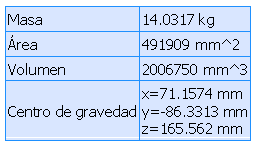
\includegraphics[scale=.95]{prop1.png}
\end{center}
\caption{Propiedades del brazo arrojadas por el software.}
\label{tabla1}:
\end{figure}

\begin{figure}
\begin{center}
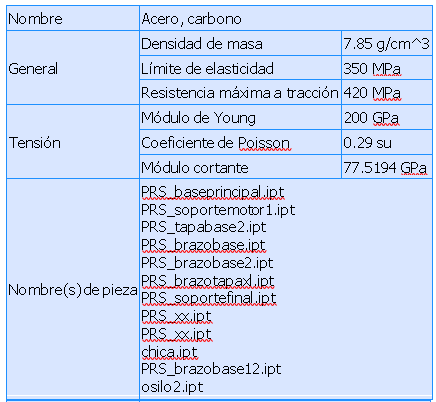
\includegraphics[scale=.85]{acero1.png}
\end{center}
\caption{Lista con las propiedades del acero y piezas que están compuestas de dicho material.}
\label{tabla2}:
\end{figure}

\begin{figure}
\begin{center}
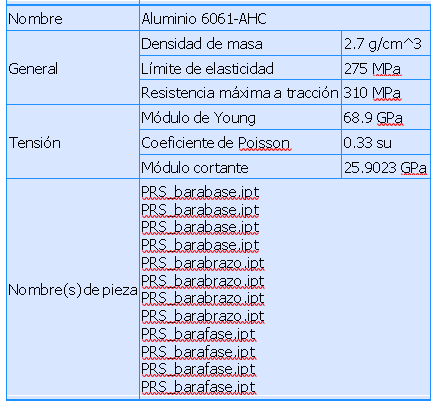
\includegraphics[scale=.85]{aluminio1.png}
\end{center}
\caption{Lista con las propiedades del aluminio y piezas que están compuestas de dicho material.}
\label{tabla3}:
\end{figure}

\end{flushleft}

\chapter{Segunda prueba}
\begin{flushleft}

\textit{"Placas de aluminio y barras de acero"}\\
Al administrar de una manera más óptima la selección de materiales para cada componente, se decidió utilizar el aluminio, un material menos denso y pesado que el acero, para la composición de las piezas de mayor volumen en el brazo y las piezas críticas, como las barras de soporte, se utilizará acero, siendo este un material más resistente. \\

Con esta configuración se crea un equilibrio entre los materiales, dejando en menor cantidad el material más denso, pero en partes donde se requiere resistencia, y los materiales livianos para el resto de las piezas del brazo.\\
El resultado de este cambio no solo beneficia en el hecho de que ya no tiene tanta deformación el brazo, sino que también el peso es disminuido con respecto al análisis previo.\\

Propiedades físicas de la segunda prueba:

\begin{figure}
\begin{center}
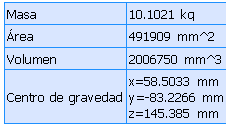
\includegraphics[scale=.95]{prop2.png}
\end{center}
\caption{Propiedades del brazo arrojadas por el software.}
\label{tabla4}:
\end{figure}

\begin{figure}
\begin{center}
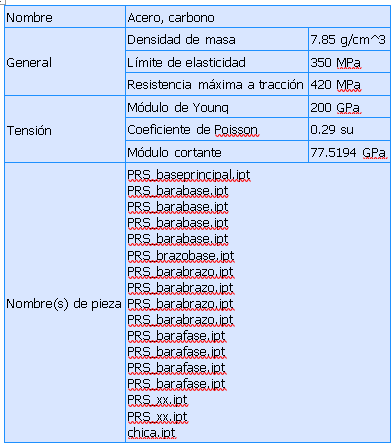
\includegraphics[scale=.85]{acero2.png}
\end{center}
\caption{Lista con las propiedades del acero y piezas que están compuestas de dicho material.}
\label{tabla5}:
\end{figure}

\begin{figure}
\begin{center}
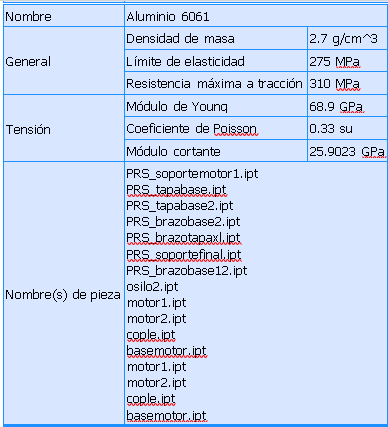
\includegraphics[scale=.85]{aluminio2.png}
\end{center}
\caption{Lista con las propiedades del aluminio y piezas que están compuestas de dicho material.}
\label{tabla6}:
\end{figure}

\end{flushleft}

\chapter{Cargas}

\begin{flushleft}

A continuación se presenta de manera gráfica la aplicación de cargas sobre la estructura del robot:

\begin{figure}
\begin{center}
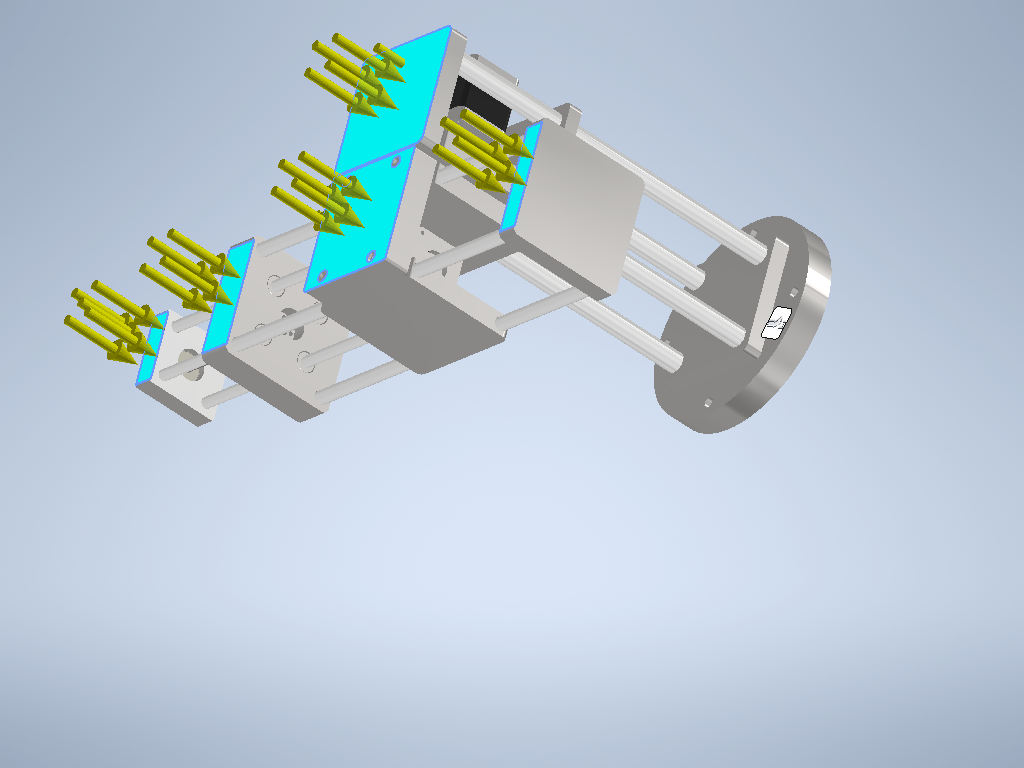
\includegraphics[scale=.55]{c1.png} 
\end{center}
\caption{Vista general con simbolización de cargas ejercidas.}
\label{tabla7}:
\end{figure}

\begin{figure}
\begin{center}
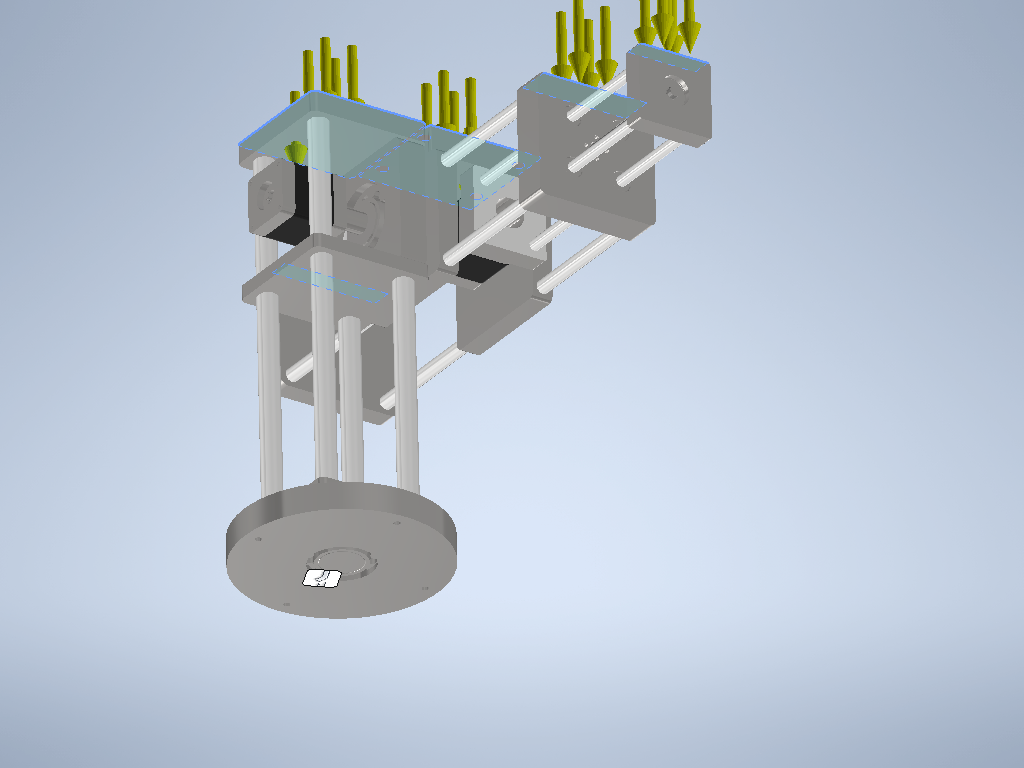
\includegraphics[scale=.55]{c2.png} 
\end{center}
\caption{Vista general desde otro ángulo con simbolización de cargas ejercidas.}
\label{tabla8}:
\end{figure}

\end{flushleft}

\chapter{Cargas en primera prueba}

\begin{flushleft}

\begin{figure}
\begin{center}
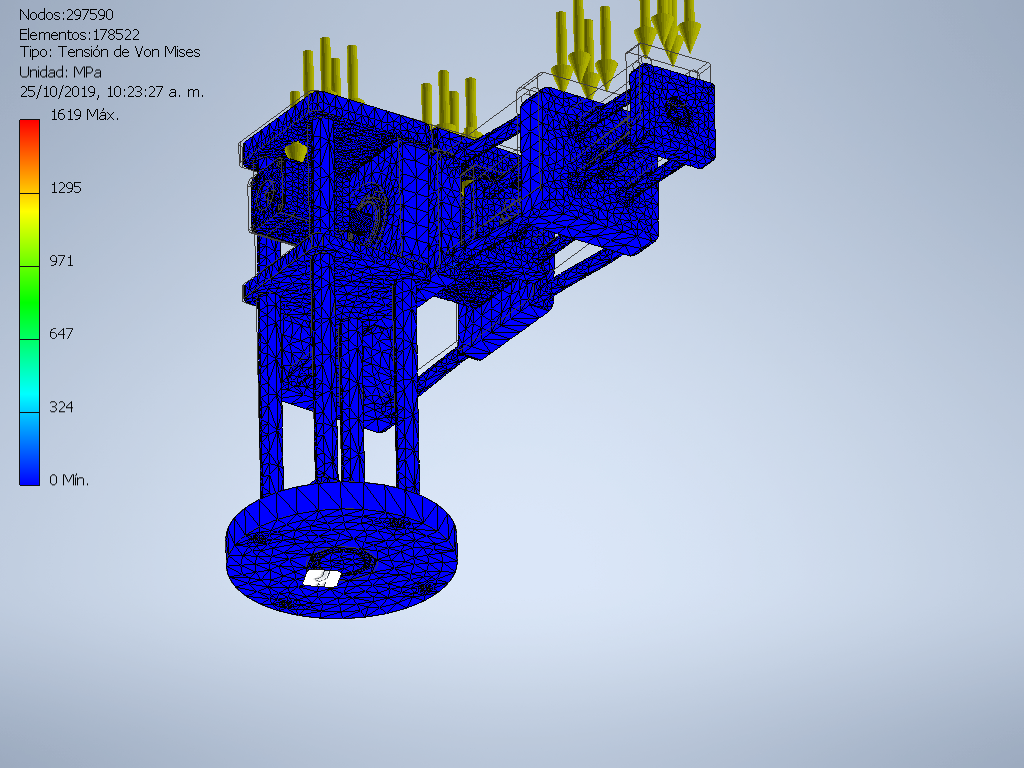
\includegraphics[scale=.55]{ca1.png}  
\end{center}
\caption{Vista general con simbolización de cargas ejercidas y desfasamiento con respecto a la posición original.}
\label{tabla9}:
\end{figure}

\begin{figure}
\begin{center}
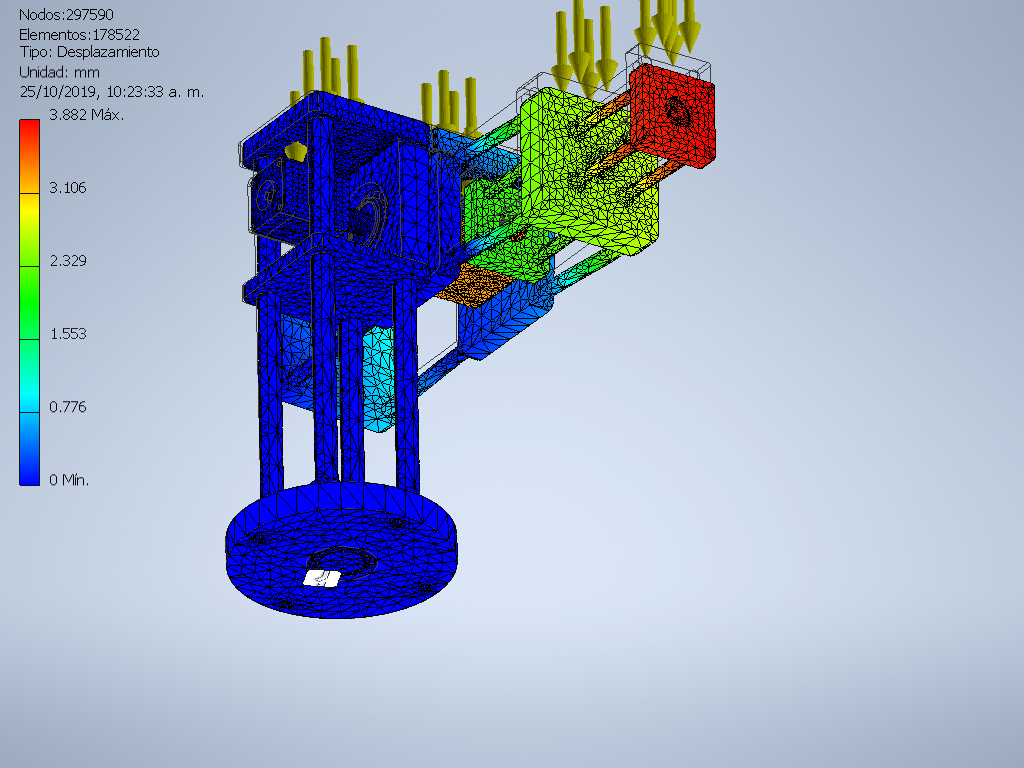
\includegraphics[scale=.55]{ca2.png}  
\end{center}
\caption{Vista general con simbolización de cargas ejercidas y colorimetría sobre las áreas de presión.}
\label{tabla10}:
\end{figure}

\begin{figure}
\begin{center}
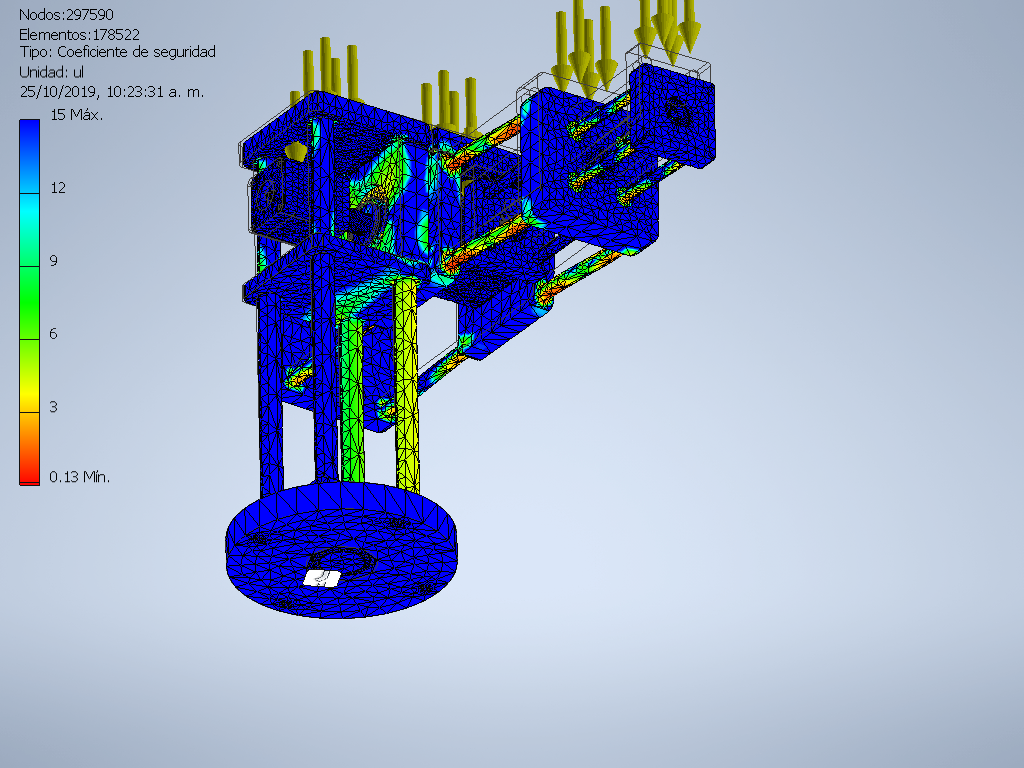
\includegraphics[scale=.55]{ca3.png}
\end{center}
\caption{Vista general con simbolización de cargas ejercidas y colorimetría sobre las áreas de deformación.}
\label{tabla11}:
\end{figure}

Como se puede notar, en esta configuración de materiales se puede observar los puntos de deterioro en la estructura del brazo, principalmente en las barras de soporte, esto debido a lo previamente mencionado de la “poca rigidez” que presenta el aluminio con el peso del robot más la carga.

\end{flushleft}

\chapter{Cargas en segunda prueba}

\begin{flushleft}

\begin{figure}
\begin{center}
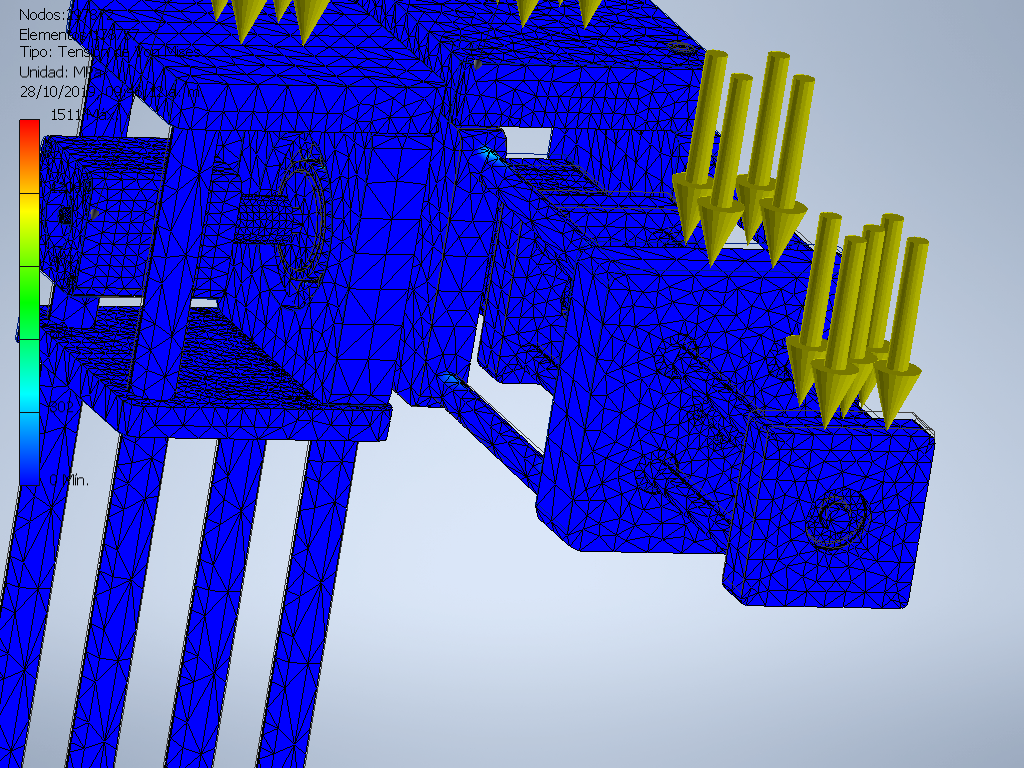
\includegraphics[scale=.55]{cb1.png}
\end{center}
\caption{Vista general con simbolización de cargas ejercidas y desfasamiento con respecto a la posición original.}
\label{tabla12}:
\end{figure}

\begin{figure}
\begin{center}
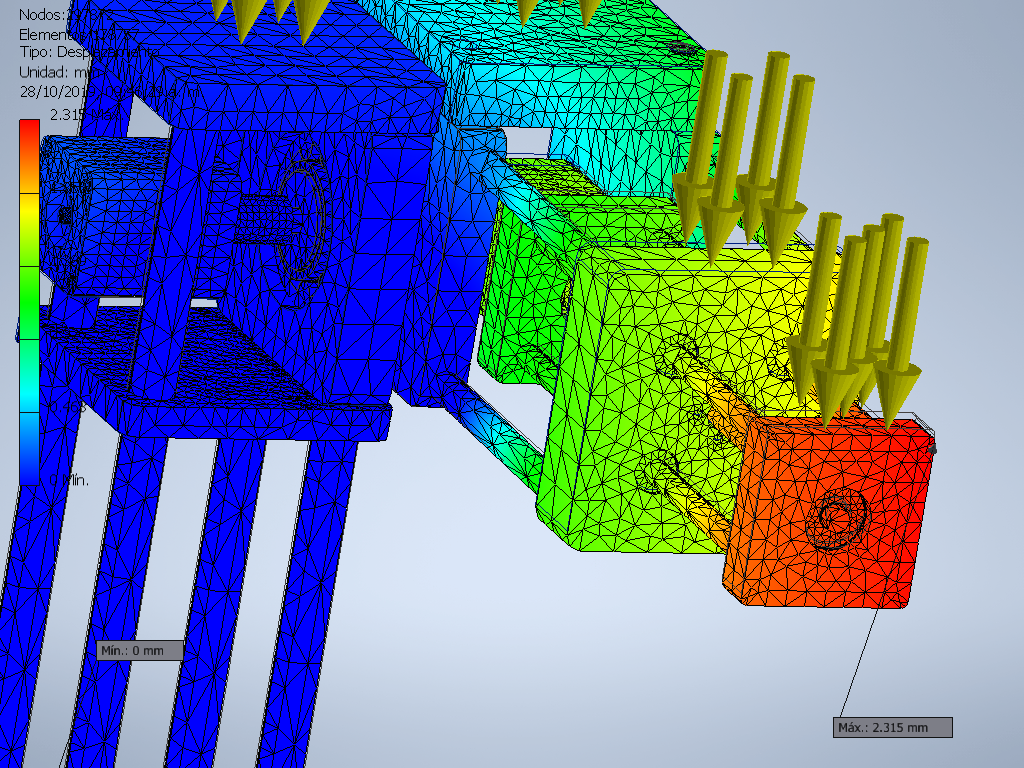
\includegraphics[scale=.55]{cb2.png}
\end{center}
\caption{Vista general con simbolización de cargas ejercidas y colorimetría sobre las áreas de presión.}
\label{tabla13}:
\end{figure}

\begin{figure}
\begin{center}
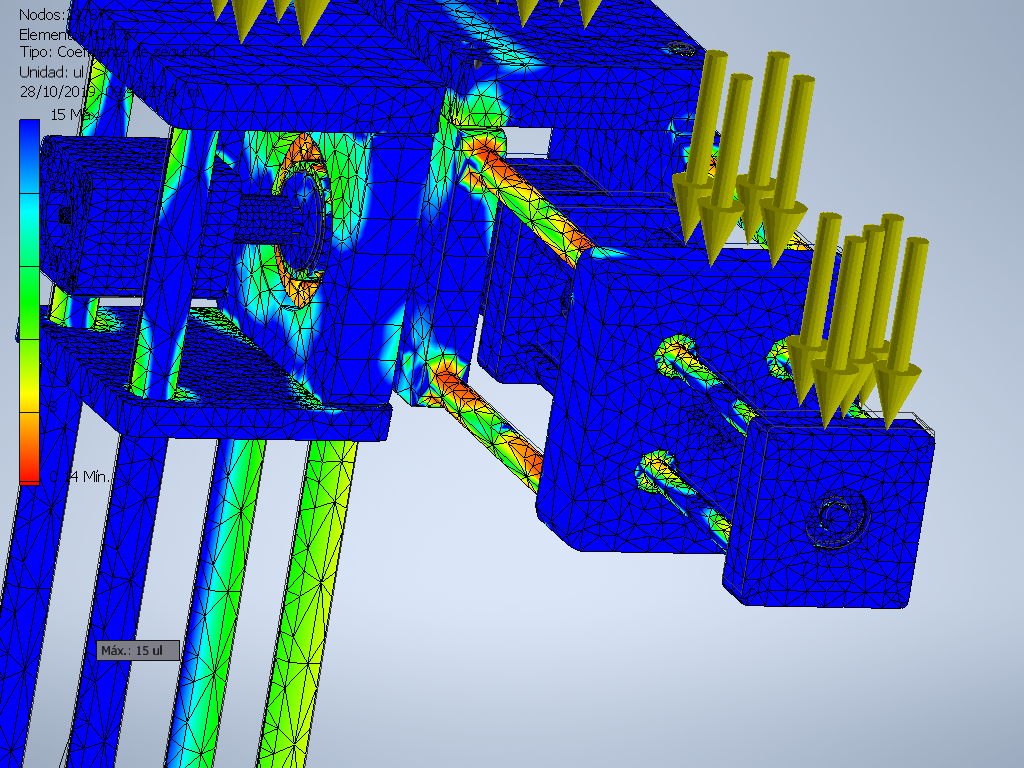
\includegraphics[scale=.55]{cb3.png} 
\end{center}
\caption{Vista general con simbolización de cargas ejercidas y colorimetría sobre las áreas de deformación.}
\label{tabla14}:
\end{figure}

\begin{figure}
\begin{center}
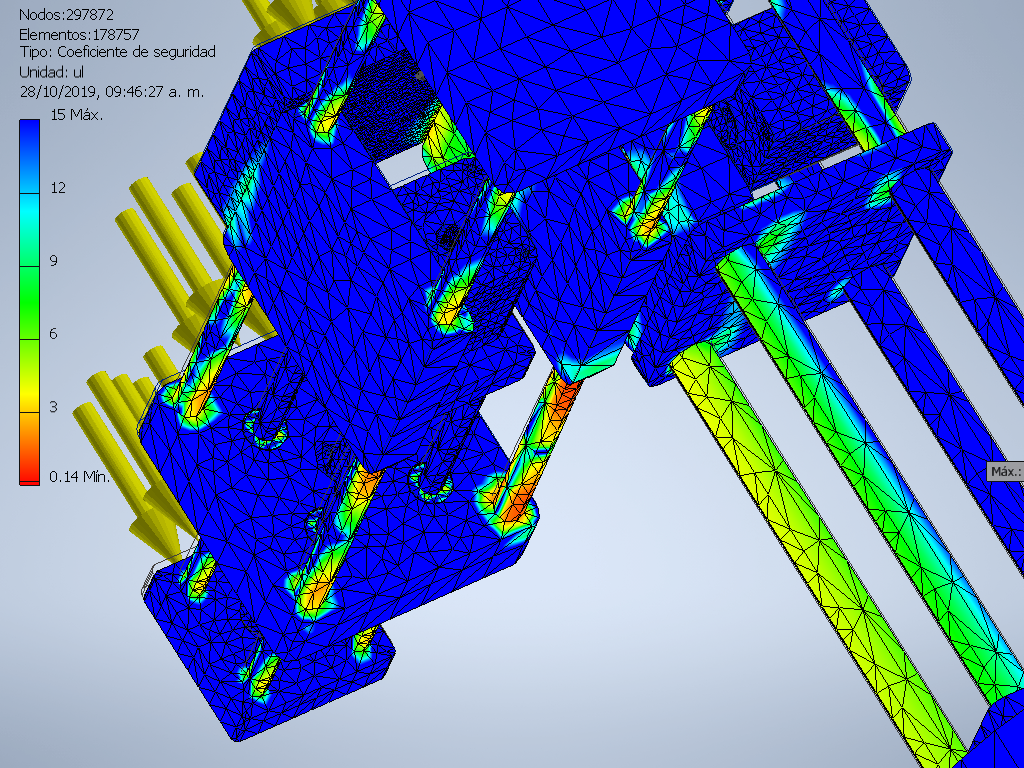
\includegraphics[scale=.55]{cb4.png} 
\end{center}
\caption{Vista general desde otro ángulo con simbolización de cargas ejercidas y colorimetría sobre las áreas de deformación.}
\label{tabla15}:
\end{figure}

Aquí podemos decir que el brazo se encuentra en condiciones más óptimas comparándolo con la versión anterior con otra configuración de materiales, el nivel de deformidad es muchísimo menos notorio, a pesar de aún presentar leves deformidades a menor escala, nuestro siguiente paso a corregir este problema es aumentar en grosor las barras de soporte, para así, darle una mayor firmeza al brazo.

\end{flushleft}

\vspace{2cm}
\hfill

\bibliographystyle{unsrt}
\bibliography{prueba}
\end{document}

}